\documentclass[onecolumn, draftclsnofoot,10pt, compsoc]{IEEEtran}
\usepackage{graphicx}
\usepackage{url}
\usepackage{setspace}
\usepackage{caption}
\usepackage{subcaption}
\usepackage{listings}
\usepackage{color}
 
\definecolor{codegreen}{rgb}{0,0.6,0}
\definecolor{codegray}{rgb}{0.5,0.5,0.5}
\definecolor{codepurple}{rgb}{0.58,0,0.82}
\definecolor{backcolour}{rgb}{0.95,0.95,0.92}
 
\lstdefinestyle{mystyle}{
backgroundcolor=\color{backcolour},   
commentstyle=\color{codegreen},
keywordstyle=\color{magenta},
numberstyle=\tiny\color{codegray},
stringstyle=\color{codepurple},
basicstyle=\footnotesize,
breakatwhitespace=false,         
breaklines=true,                 
captionpos=b,                    
keepspaces=true,                 
numbers=left,                    
numbersep=5pt,                  
showspaces=false,                
showstringspaces=false,
showtabs=false,                  
tabsize=2
}
 
\lstset{style=mystyle}
\graphicspath{ {Images/} }
\usepackage{geometry}
\usepackage{imakeidx}
\makeindex[columns=1, options=-s lou3.ist]
\geometry{textheight=9.5in, textwidth=7in}

% 1. Fill in these details
\def \CapstoneTeamName{   The Visionaries}
\def \CapstoneTeamNumber{   3}
\def \GroupMemberOne{     Kien Tran}
\def \GroupMemberTwo{       Brian Wiltse}
\def \CapstoneProjectName{    Code3 Visionary}
\def \CapstoneSponsorCompany{ Levrum Data Technologies}
\def \CapstoneSponsorPerson{  Carl Niedner}

% 2. Uncomment the appropriate line below so that the document type works
\def \DocType{    
        %Requirements Document
        % Review
        %Design Document
        Progress Report
        }
      
\newcommand{\NameSigPair}[1]{\par
\makebox[2.75in][r]{#1} \hfil   \makebox[3.25in]{\makebox[2.25in]{\hrulefill} \hfill    \makebox[.75in]{\hrulefill}}
\par\vspace{-12pt} \textit{\tiny\noindent
\makebox[2.75in]{} \hfil    \makebox[3.25in]{\makebox[2.25in][r]{Signature} \hfill  \makebox[.75in][r]{Date}}}}
\newcommand{\tabitem}{~~\llap{\textbullet}~~}
% 3. If the document is not to be signed, uncomment the RENEWcommand below
\renewcommand{\NameSigPair}[1]{#1}

%%%%%%%%%%%%%%%%%%%%%%%%%%%%%%%%%%%%%%%
\begin{document}

\begin{titlepage}
    \pagenumbering{gobble}
    \begin{singlespace}
      
\includegraphics[height=4cm]{coe_v_spot1}
        \hfill 
        % 4. If you have a logo, use this include graphics command to put it on the cover sheet.
        %\includegraphics[height=4cm]{CompanyLogo}   
        \par\vspace{.2in}
        \centering
        \scshape{
            \huge CS Capstone \DocType \par
            \large{Spring Term}\par
            {\large\today}\par
            \vspace{.5in}
            \textbf{\Huge\CapstoneProjectName}\par
            \vfill
            {\large Prepared for}\par
            \Huge \CapstoneSponsorCompany\par
            \vspace{5pt}
            {\Large\NameSigPair{\CapstoneSponsorPerson}\par}
            {\large Prepared by }\par
            Group\CapstoneTeamNumber\par
            % 5. comment out the line below this one if you do not wish to name your team
            \CapstoneTeamName\par 
            \vspace{5pt}
            {\Large
                \NameSigPair{\GroupMemberOne}\par
                \NameSigPair{\GroupMemberTwo}\par
            }
            \vspace{20pt}
        }
        \begin{abstract}
                Over the last five weeks, our team has continued to work on Code3 Visionary.
                Though our project requirements have changed rapidly over the course of the class, the underlying purpose remains the same as when we began: Code3 Visionary (C3V) aims to predict emergency incident density in a given time and place. 
                The scope of C3V, and our contribution to it, is now clearly defined. 
                C3V is a set of tools designed to generate a correlational model between incident density within Charlotte, NC, and the attributes of those areas.
                This report provides an overview of our progress on the project, emphasizing the beginning of Spring Term, and what work is yet to be done. 
        \end{abstract}
    \end{singlespace}
\end{titlepage}
\newpage
\pagenumbering{arabic}
\tableofcontents
% 7. uncomment this (if applicable). Consider adding a page break.
\listoffigures
\listoftables
\lstlistoflistings
\clearpage

% 8. now you write!
\section{Introduction}
\begin{singlespace}
Our project, Code3 Visionary (C3V), is an application designed to predict how many emergency calls, and what types of emergency calls, will occur in a given time and place. 
C3V involves gathering data, researching and implementing a machine learning algorithm, building an API, and building a minimal user interface that can display C3V's results. 

As we mentioned in our prior progress reports, Code3 Visionary is a collaborative project with software engineers at Levrum, and our project specifications have been subject to change depending on the needs of the Levrum team. 
Now, as we near the Undergraduate Engineering Expo, we are finalizing all of the aspects of the project we have been able to work on.
Our original project documentation discussed C3V in broad terms in order to provide a general concept of what Levrum and we were hoping to accomplish. 
This term so far has consisted of adding new features to provide Levrum with as thorough an analysis as possible and, more recently, cleaning up our code base and revising our documentation to describe the work we have contributed. 

The remainder of this document provides an overview of the status of our project's components.
Further, we discuss the work that is yet to be done on all aspects of our project.
Section \ref{expo} discusses our status in preparing for Expo.
Section \ref{docs} discusses the status of our Requirements and Design documentation.
Section \ref{tools} provides an overview of each of our project deliverables. 
We summarize our challenges in Section \ref{challenges}.
Finally, we conclude with Section \ref{conclusion}, which includes a summary of work we have yet to do.

\end{singlespace}

\section{Expo Preparation} \label{expo}
\begin{singlespace}
We have completed all administrative steps to prepare for Expo on May 18.
Our registration is complete, and our poster and model release forms are submitted; all steps were completed on-time.

As far as preparation for the day itself, we have prepared our so-called elevator pitch, the low-tech version of which is presented in the accompanying presentation. 
One task we have yet to do is prepare a set of visuals to illustrate our process of obtaining data and visualizing our analyses.
We have requested a monitor and power supply for these visuals, and we have plenty of visuals to use, but we have yet to organize the visuals for presentation.
\end{singlespace}

\section{Documentation} \label{docs}
\begin{singlespace}
We have recently made revisions to our documentation to reflect the work we have accomplished on the project. As of the time of this writing, Carl Niedner, our project sponsor, has approved of the revisions and has sent a sign-off email to our TA and the instructors of the course. The documentation should be complete and in its final form. We do not anticipate having to make any further changes; however we have not heard feedback from our TA or instructors yet.
\end{singlespace}

\section{Deliverables} \label{tools}
\begin{singlespace}

\subsection{Data Ingestion and Feature Extraction}
The data ingestion and feature extraction tool is feature-complete. 
The tool has undergone considerable revision over the course of the project as our skills and our knowledge of Python's data science libraries have grown.
As outlined in our most recent documentation, the tool compiles and performs various calculations in order to output a ready-for-analysis data set. Details of many of the components have been discussed in prior progress reports. Here, we will describe features we have added this term and illustrate how they contribute to some of the system attributes outlined in our requirements and design documents.

Listing \ref{lst:density} illustrates a simple feature extraction example. Note that computing the density of population and employment is a simple calculation performed on entire columns of the input dataframe. Taking advantage of the Pandas library to divide over columns makes the code simple, easy to understand, and performant. When we first began work on this project, we used for-loops for similar operations, which were often much slower and introduced opportunities for errors.

\begin{lstlisting}[language=Python, caption={Extracting population and employment density from raw data},label={lst:density}, captionpos=b]
from __future__ import division


def get_densities(gdf, target_columns, area_column, drop=False):
    """
    Returns a GeoDataFrame with densities given by each target_column divided by the designated area_column.
    :param gdf: A GeoDataFrame
    :param target_columns: A list of columns for which to find densities
    :param drop: True if the columns used for feature extraction should be dropped after calculations.
    Defaults to False
    :return: GeoDataFrame Population / Unit of area
    """
    for col_label in target_columns:
        new_label = col_label[:9] + '%'
        gdf[new_label] = gdf[col_label] / gdf[area_column]

    if drop:
        gdf.drop(columns=target_columns, inplace=True)

    return gdf
\end{lstlisting} 

Listing \ref{lst:zones} illustrates the same concept with a more complex operation. Levrum determined that zoning information was important to include in our feature set, but wanted to combine some zones into higher-level categories. For example, instead of distinguishing between single-family and multiple-family residence zones, Levrum wanted to combine them into a single ``residential" category. We again take advantage of the Pandas dataframe to perform the sum operation over entire columns in $sum\_cols()$. In the function $sum\_combine\_columns()$,  we $reduce()$ the lists of original columns using $sum\_cols()$ and map them to their new categories.

\begin{lstlisting}[language=Python, caption={Combining zone proportions into higher-level zones.}, label={lst:zones}, captionpos=b]
def sum_cols(a, b):
    """
    Sums two (Geo)Series (columns in a DataFrame) 
    :param a: A Series (DataFrame column) to combine
    :param b: Another Series to combine
    :return: A combined column with summed elements
    """
    return a.combine(b, lambda s1, s2: s1 + s2)


def sum_combine_columns(df, col_dict):
    """
    Creates columns that represent a sum of existing columns in a given DataFrame.
    :param df: Dataframe to modify
    :param col_dict: Dict mapping {New_column: [old_col1, old_col2, ...]
    :return: Dataframe with old columns summed into new columns
    """
    for new_col, lst in col_dict.iteritems():
        df[new_col] = reduce(sum_cols, [df[col] for col in lst])

    df.drop([el for lst in col_dict.itervalues() for el in lst], axis=1, inplace=True)

    return df
\end{lstlisting}

Both of these examples attest to these modules' extensibility and modifiability. Both modules were created independently and inserted into the data pipeline of our program. Listing \ref{lst:pipeline} shows how the module to combine zones into higher-level categories was inserted into the pipeline. After the preexisting functionality of obtaining the zone proportions is completed, we pass the resulting dataframe, along with a map describing how to combine the zones, into the new module. The new module returns the modified dataframe and the work flow continues as before. This pipeline structure also contributes to the modules' testability. Both modules have their own individual tests to ensure the results come out as expected.

\begin{lstlisting}[language=Python, caption={Inserting the new zone-combination module into the pipeline.}, label={lst:pipeline}, captionpos=b]
    ...
    if zone:
        zone_gdf = gpd.read_file(Names.get_zoning_shapefile(state_code=state_code,                                      county_code=county_code, year=year))
        
        # Obtain zone proportions
        gdf = GetZoningData.combine_zones(base_gdf=gdf, zone_gdf=zone_gdf, base_shp_col=base_shape)

        # Create higher level zone categories
        zones_to_combine = \
            {
                'RESIDENTIAL': ['SINGLE FAMILY', 'MULTI-FAMILY'],
                'COMMERCIAL': ['OFFICE', 'BUSINESS', 'MIXED USE']
            }

        gdf = CombineColumns.sum_combine_columns(gdf, zones_to_combine)
    ...
\end{lstlisting}

Further, each step of the process is tested with either unit or integration tests or both. 
Current testing fulfills the requirements of our documentation; however, we want to supplement the current testing with a more comprehensive integration test. In addition, a test for gathering U.S. Census demographics from a random place and time was broken during a revision earlier in the year. We have not addressed the test because the data ingestion and feature extraction tool has only been applied to Charlotte, NC so far. We do, however, need to fix the test before finalizing the project.


\subsection{K-means (Extra)}
We were able to utilize another machine learning tool, K-means, to help with our analysis. K-means is an algorithm that projects the features of our data set into multi-dimensional space and attempts to find data points that cluster together. Clusters are formed by moving an arbitrary number (K) of centroids among the projected samples until the distances between samples and their closest centroid are minimized. The clusters represent samples, which are TAZs in our case, that group together by their combined features. Figure \ref{fig:clusters} shows a clustering with $K = 6$ centroids.

\begin{figure}[h!]
    \centering
    \includegraphics[scale=0.25]{clusters.eps}
    \caption{K-means clustering ($K=6$) of our data set.}
    \label{fig:clusters}
\end{figure}

Levrum can use this information by running our analysis module on the clusters, rather than each TAZ individually. If the clusters represent a good grouping of the data, then we hope that we can find even stronger correlations between incident densities and clusters. Our K-means code is set up to run with an arbitrary number of clusters. Further, we have an option to perform principal component analysis (PCA), which reduces the dimensionality of our data by combining features that are most strongly correlated, before running K-means. We have provided Levrum with K-means data with and without PCA.

% ------------------------------ REMINDERS ------------------------------------
% Your group REPORT:
%   briefly recaps the project purposes and goals
%   describes where you are currently on the project
%   describes what you have left to do
%   describes any problems that have impeded your progress, with any solutions you have
%   includes particularly interesting pieces of code (if coding is involved)
%   includes images of your project -- screen shots, photos, whatever is appropriate
%   Clarity of thought, presentation, spelling, and grammar will all be evaluated for grading purposes. Please ensure you take this document seriously.


\subsection{Machine Learning and Analysis}\label{ml}
% Kien
For machine learning we opted to use a genetic algorithm in order to help us select features from our data set.
Due our data set containing  multiple categories/features, it would have taken \(2^n\) time complexity to brute force all combinations of features.
We needed a way to find the best combination of these features in order to run geographic weighted regression (GWR) on the selected features.
The best combination of features would have the highest adjusted correlation of determination to be used as a model for predicting the future call sets.

Genetic algorithm (GA) is method of feature selection using biology-inspired methods such as mutation, cross-over, and multiple generations. It starts by first creating a pre-selected amount of individuals with some features turned on (1) and some turned off (0). 
These features are randomized for each individuals during assignment and all of them together is known as a pool. 
After we created our pool, we would run a regression model test on each individuals to rate their fitness.
The ones with the highest fitness (highest coefficient of determination) will be paired with others with high fitness in order to create a new generation of individuals with the best combinations of features.
This is done over a predetermined amount of generations, and the individual with the highest fitness will have their features outputted by the algorithm for the users to see.
Following the crossover of individuals, we also implemented a mutation factor that randomly turns a feature on or off.
This mutation factor is set by the user to make sure we do not miss key combinations that would have never been discovered with simple crossover generations.

Listing 4 showcases the options we have available for the user to change as well as the internal variables we have set for our GA algorithm.
Changing the iterations will allow the GA to run for more or fewer generations and the pool size dictates the amount of individuals created for each generation.
To ensure that our algorithm does not take too long, we've settled on running for only 100 generations at a rate of 50 individuals per generations.
The time it takes to run this on a 60 feature data set is down to less than a minute.

\begin{lstlisting}[language=Python, caption={Initial setup for genetic algorithm.}, label={lst:GA}, captionpos=b]
    ...
   class FeatureSelectionGeneticAlgorithm():
    # Initialize state, setting up:
    #    + mutation rate - Number controlling the chance of mutation (between 0 - 1)
    #    + iterations - Controls the number of generations the algorithm will create
    #    + pool_size - Population that the algorithm will consider in each generations
    def __init__(self, mutation_rate = 0.01, iterations = 100, pool_size = 50):
        self.mutation_rate = mutation_rate
        self.iterations = iterations
        self.pool_size = pool_size
        self.pool = np.array([])
        self.iterations_results = {}
        self.r2_li = []
        self.r2_adj = []
        self.kf = KFold(n_splits = 5)
    ...
\end{lstlisting}

Figure 2 showcases our graph of the GA score and how it performed over multiple generations.
The scores acted like how we expected; it began at a low rate early on and then after a few generations it rose quickly.
Over time the score will stagnate due to the algorithm already finding the best features, which is when our mutation rate applies variance to the selected features.
If the mutation resulted in a good score, we would see the line shift a level up, however, if it is a bad feature the score will go down temporarily but will be brought back up by the next generation.

\begin{figure}[h!]
    \centering
    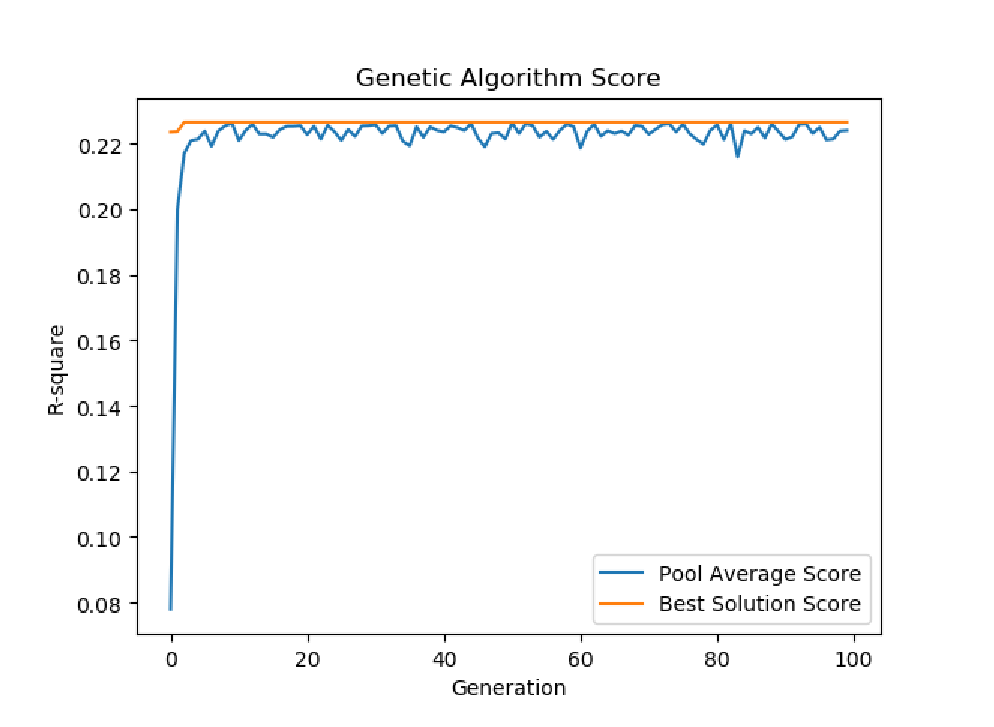
\includegraphics[scale=0.5]{GA.eps}
    \caption{Genetic Algorithm of data set ($pool size = 50, generations = 100, mutation-rate = 0.01$).}
    \label{fig:GA}
\end{figure}

Once the feature is chosen, we run the set of features through our GWR algorithm to calculate the adjusted R-squared for the call set with the optimal features selected.
GWR uses separate equations for each feature in a data set in order to calculate the correlation of determination for the entire set.
It utilizes spatial data to find out who its neighboring features are and calculates based off those neighbors.
This is done through calling an R-script which has GWR already implemented.
We use python to first setup the necessary components/files and then those to the R-script for calculations.
Listing 5 showcases how we constructed the R-script and send it the arguments that it needs.

\begin{lstlisting}[language=Python, caption={Initial setup for GWR.}, label={lst:GWR}, captionpos=b]
    ...
    #Creates a dataframe using pandas with the already calculated values
    df = pd.DataFrame({'Calls':listcall, 'Latitude':listlat, 'Longtitude':listlong, 'x':xcords, 'y':ycords})
    num = 0
    for name in listname:
        df.insert(0,name,primarylist[num])
        num=num+1
    df.to_csv('temp.csv', sep=',')



    #Run R Script as a subprocess
    R_script = 'example_script.R'
    cmd = ['Rscript', R_script] + listname
    x = subprocess.check_output(cmd, universal_newlines=True)
    ...
\end{lstlisting}

When the best set of features is determined, we use those set of features as the predictors in our prediction model and supply it with a projection of future demographic data to predict on.
More testing on the algorithm is needed to make sure it runs correctly and outputs the results we are expecting.

\subsection{API} \label{api}
% Kien

The API uses Google's App Engine to setup a REST API.
The REST API utilizes POST and GET requests in order to upload and retrieve the future predicted calls that we will be outputting.
For the POST request, users must supply in the body, the "year", "location", "callcount", and (optionally) "cause".
These values will be stored in a NoSQL database locally or on Google's servers when the app is launched. 
With the GET request, the user will need to supply, the "year", "location", and "cause" and the algorithm will return a JSON object with the number of predicted calls that matches those variables.
Listing 6 showcases our NoSQL database and the type of properties each entry holds.

\begin{lstlisting}[language=Python, caption={API NoSQL database.}, label={lst:API}, captionpos=b]
    ...
    class predictCalls(ndb.Model):
	    id=ndb.StringProperty()
	    cause=ndb.StringProperty()
	    year=ndb.IntegerProperty(required=True)
	    location=ndb.IntegerProperty(required=True)
	    callcount=ndb.IntegerProperty(required=True)
    ...
\end{lstlisting}

The application programming interface is very basic at this time and will require more testing to confirm that the data we upload is the same when we retrieve.
We would also like to implement a DEL function to get rid of entries that are no longer relevant or have been updated.

\section{Challenges} \label{challenges}
By far the most challenging aspect of this project has been keeping up with quickly changing requirements at Levrum and ensuring that, while doing so, we were meeting the requirements of the Capstone class. The week preceding the submission of this report required a significant investment of time to rewrite our documentation to reflect the actual work we completed on the project. The week before that involved making substantial modifications to our poster for the same purpose. We did not simply put off the changes; we found that making modifications to our documentation for each change took too much time away from actual work on the project. Moreover, submitting version after version of the documentation likely would have annoyed all involved in signing off on the changes.

Other than the requirements challenges, we have been pushing ourselves to learn as much as possible about all of processes our project entails. Both of us have had to gain significantly more knowledge of data science over the course of the project.  

\section{Conclusion} \label{conclusion}
This report has provided an overview of our project's status, our challenges, and our next steps. We are happy to report that project is nearly finished and ready to present at Expo. We have mentioned the tasks that we intend to complete throughout this report, and these items are listed in Table \ref{tab:Todo}.


\begin{center}
\captionof{table}{\textbf{To Do Items}} \label{tab:Todo}
\begin{singlespace}
\begin{tabular}{ |p{0.75\linewidth}| }
    \hline
     \\
     \tabitem Fix randomized test for Census demographic module in the data ingestion tool.
     \\
     \tabitem Improve documentation of data ingestion tool.
     \\
     \tabitem Compile a set of visuals for presentation at Expo.
     \\
     \tabitem Perform analysis on K-Means clusters (stretch goal).
     \\
	 \tabitem Add end-to-end tests for data ingestion tool (stretch goal).
     \\
     \tabitem Add unit testing for genetic algorithm and API.
     \\
     \tabitem Implement DELETE and PATCH requests to API.
     \\
     \hline
\end{tabular}
\end{singlespace}
\end{center}


\end{singlespace}
% REFERENCES
%\newpage    
%\bibliography{WMidtermRepRef}{}
%\bibliographystyle{ieeetr}

\end{document}


